% Dans l'introduction, on présente le problème étudié et les buts
% poursuivis. L'introduction permet de faire connaître le cadre de la
% recherche et d'en préciser le domaine d'application. Elle fournit
% les précisions nécessaires en ce qui concerne le contexte de
% réalisation de la recherche, l'approche envisagée, l'évolution de
% la réalisation. En fait, l'introduction présente au lecteur ce
% qu'il doit savoir pour comprendre la recherche et en connaître la
% portée.
\Chapter{INTRODUCTION}\label{sec:Introduction}  % 10-12 lignes pour introduire le sujet.
Les processus de diffusion occupent une place centrale en finance pour modéliser l'évolution temporelle d'une grande variété d'instruments financiers. Parmi les problématiques associées à ces modèles, l'étude des \textit{temps de premier passage} revêt une importance particulière, notamment en gestion des risques, en évaluation d'options barrières ou encore en prévision d'événements extrêmes.\\
Un autre aspect fondamental concerne la \textit{commande optimale stochastique}, qui consiste à influencer dynamiquement l'évolution du processus jusqu'à un temps d'arrêt, dans le but de minimiser un coût cumulé, composé d'un coût de contrôle et éventuellement d'un coût d'état.\\
Ce mémoire s'intéresse à l'analyse conjointe des temps de franchissement et de la commande optimale appliquées au processus de \acl{CIR}~\cite{cox1985}, proposé en 1985, un modèle de référence largement utilisé pour représenter la dynamique des taux d'intérêt.
 
% Texte en \emph{italique}, \textsc{petites majuscules}, mot \mbox{insécable}.\\
% Texte \ul{souligné}, \hl{surligné}, \textbf{gras}.\\
% Texte entre ``guillemets''.\\
% Police \texttt{monospace}.\\
% Un mot courant en réseautique mobile: n\oe{}ud\footnote{Note de bas de page.}.\\
% L'objet RSVP \texttt{SENDER\_TEMPLATE}.\\
% %Nom d'un auteur: \citeauthor{RFC_IPv4}.\\
% Une architecture 32~bits.\\
%%
%%  CONCEPTS DE BASE / BASIC CONCEPTS
%%
\section{Définitions et concepts de base}  % environ 2-3 pages

Avant d'approfondir le sujet, il est essentiel de poser clairement les fondements théoriques sur lesquels repose cette étude.\\
L'élément central à introduire en premier lieu est le \textit{mouvement Brownien standard}, pierre angulaire des processus de diffusion.
\paragraph{Définition: Le \acl{MBS}}\mbox{}\\ 
Un processus stochastique $\{W(t),\;t\geq0\}$ est un mouvement Brownien standard s'il vérifie:
\begin{itemize}
    \item $W(0) = 0$;
    \item les trajectoires $t \mapsto W(t)$ sont continues presque sûrement;
    \item il possède des accroissements indépendants: pour tout $0 \leq t_0 < t_1 < \cdots < t_n$, les variables aléatoires ${\left(W(t_i) - W(t_{i-1})\right)}_{i=1}^n$ sont indépendantes;
    \item il possède des accroissements stationnaires gaussiens: pour tout $0 \leq s \leq t$, on a $W(t) - W(s) \sim \mathcal{N}(0, t - s)$.
\end{itemize}
\begin{figure}[htb]
    \centering
    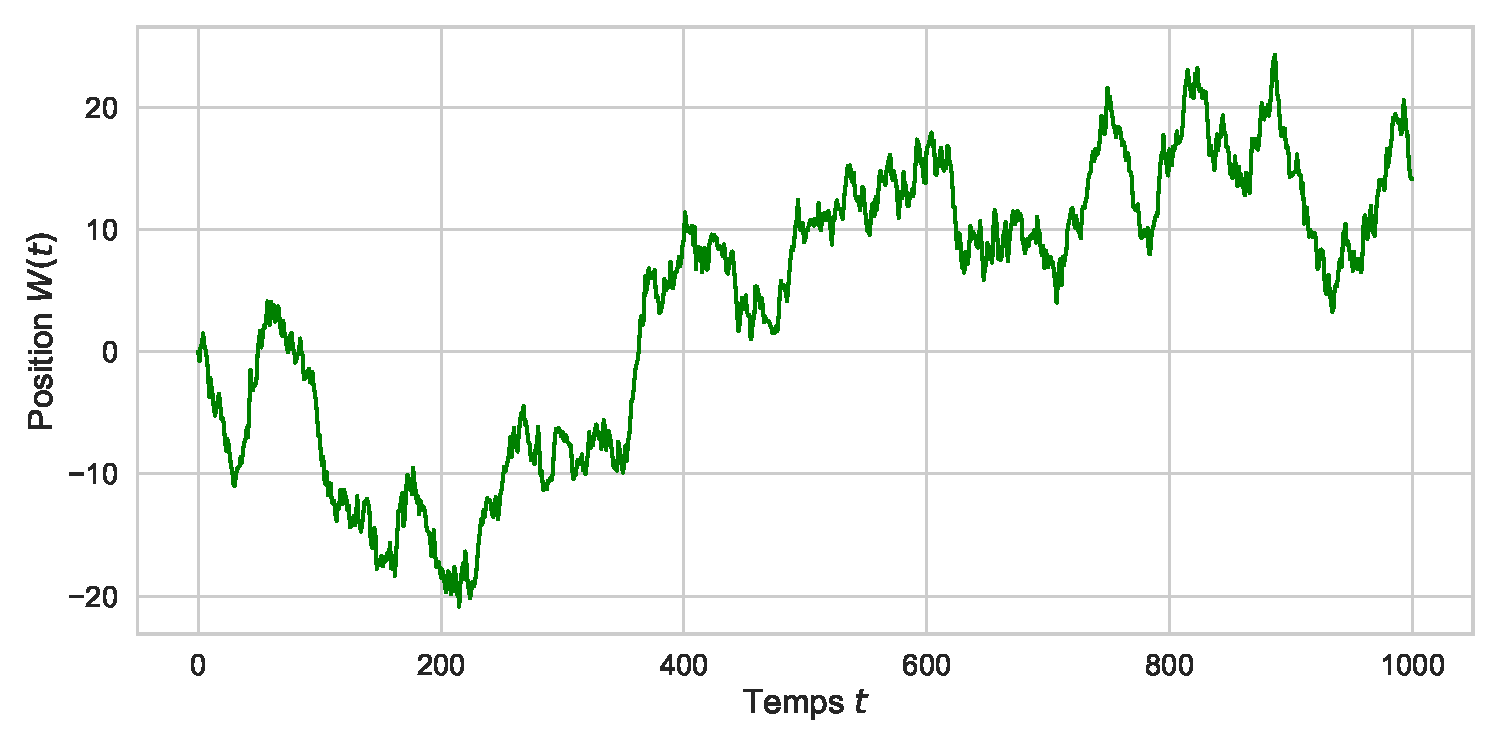
\includegraphics[width=0.9\linewidth]{img/intro/path_MBS.pdf}
    \caption{Une trajectoire du \acl{MBS}}\label{fig:TrajMBS}
\end{figure}
\FloatBarrier Le \acs{MBS} constitue la base de la construction des processus de diffusion employés dans de nombreux domaines tels que la finance, la physique ou la biologie. Ces processus sont modélisés par des \acf{EDS}, qui consistent à enrichir le mouvement brownien en y ajoutant un terme de dérive et un terme de diffusion. Il en résulte une classe de processus dits \textit{d'Itô}.
\paragraph{Définition: Processus d'Itô}\mbox{}\\
$\{X(t),\;t \geq 0\}$ est un processus d'Itô~\cite{ito1944} s'il satisfait une équation différentielle stochastique de la forme:
\begin{equation}
    dX(t) = \mu(t, X(t))\,dt + \sigma(t, X(t))\,dW(t)
\end{equation}\label{ito_eq}
où:
\begin{itemize}
    \item $\mu(t, X(t))$ et $\sigma(t, X(t))$ sont des fonctions mesurables et adaptées à la filtration brownienne standard $\mathcal{F}_t=\sigma\{W(s),\;s\leq t\}$;
    \item $\mathds{P}\left( \int_0^T |\mu(s, X(s))|\,ds < +\infty \right) = 1$;
    \item $\mathds{P}\left( \int_0^T \sigma^2(s, X(s))\,ds < +\infty \right) = 1$.
\end{itemize}
Dans cette formulation, $\mu(t, X(t))$ est appelé le \textit{terme de dérive} et $\sigma(t, X(t))$ le \textit{terme de diffusion}.
\begin{figure}[htb]
    \centering
    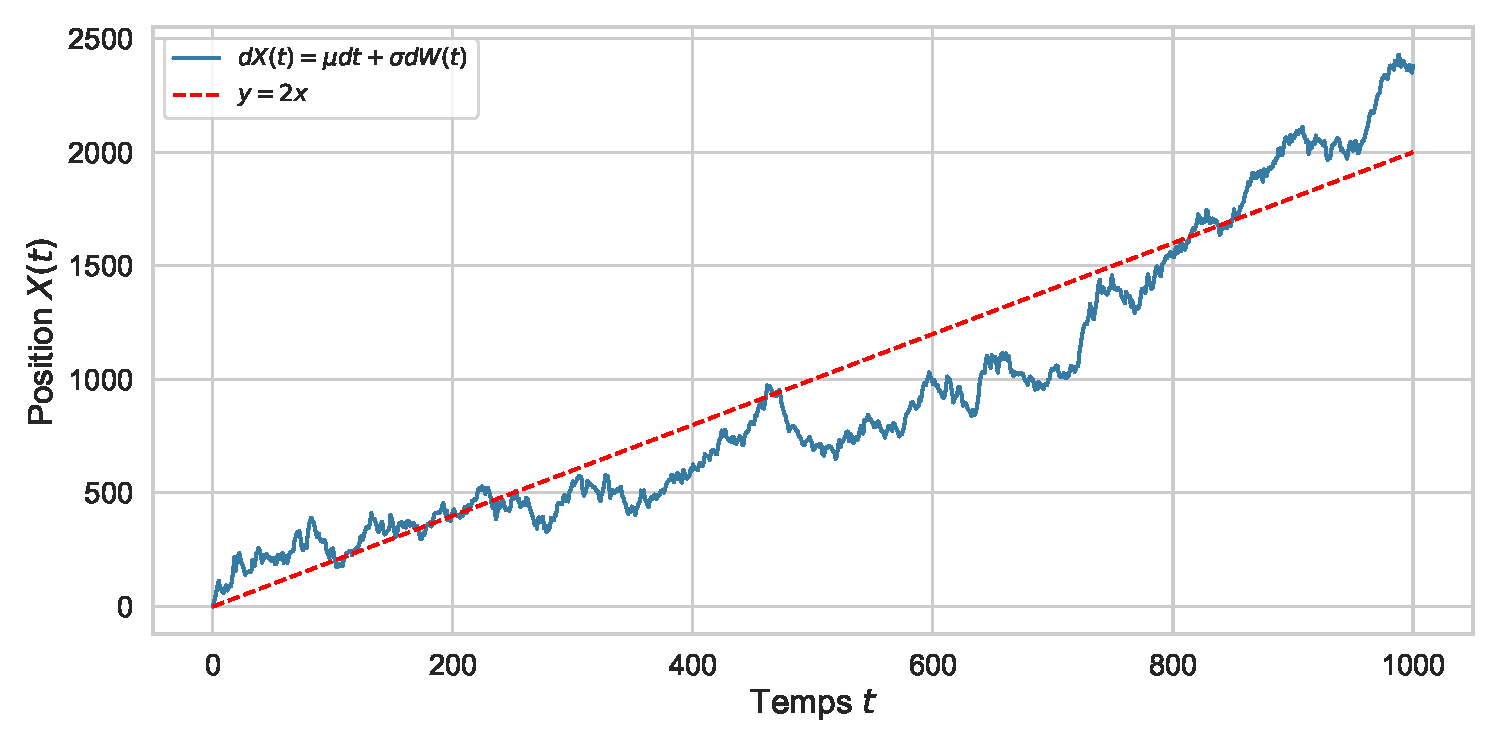
\includegraphics[width=0.9\linewidth]{img/intro/path_drift.pdf}
    \caption{Une trajectoire d'un processus d'Itô avec $\mu(t, X(t)) \equiv \mu = 2$}\label{fig:TrajIto}
\end{figure}
\FloatBarrier La figure~\ref{fig:TrajIto} illustre l'effet d'une dérive: la trajectoire du processus s'organise autour de la courbe moyenne \( y = 2x \), tout en étant perturbée par la composante aléatoire de la diffusion.

De plus, il est important de noter que les termes de dérive et de diffusion peuvent eux-mêmes dépendre de l'état du processus ou du temps, ce qui permet de capturer des dynamiques complexes, comme une volatilité ou une dérive variable. Cette flexibilité permet notamment de modéliser des phénomènes réalistes dans les systèmes financiers ou physiques.

Par ailleurs, Il est parfois intéressant d'enrichir les processus d'Itô en leur ajoutant une composante de sauts, gouvernée par un processus de Poisson (processus de comptage classique modélisant une file d'attente).
\paragraph{Définition: Processus de Poisson}\mbox{}\\
Un processus $\{N(t),\;t\geq0\}$ est un processus de Poisson de taux $\lambda$ s'il vérifie:
\begin{itemize}
    \item Pour des intervalles de temps disjoints, le nombre d'occurrences est indépendant: pour tout $0 \leq t_0 < t_1 < \cdots < t_n$, les variables aléatoires ${\left(N(t_i) - N(t_{i-1})\right)}_{i=1}^n$ sont indépendantes;
    \item La probabilité d'une occurrence dans un petit intervalle de temps dépend de la longueur de l'intervalle: $\underset{h\to0^+}{\lim}\mathds{P}[N(t+h)-N(t)=1]=\lambda h+o(h)$;
    \item La probabilité qu'il y ait plus d'une occurrence au sein d'un petit intervalle est négligeable: $\underset{h\to0^+}{\lim}\mathds{P}[N(t+h)-N(t)>1]=o(h)$;
    \item Le nombre d'occurrences dans un intervalle de longueur $t$ suit une loi poisson: $N(t)\sim \text{Poi}(\lambda t)$;
    \item Le temps d'arrivé du $n$-ème événement $T_n$ suis une loi exponentielle: $T_n\sim\text{Exp}(\lambda)$.
\end{itemize}
En utilisant un processus de Poisson, il est donc possible de définir un processus de sauts pur.
\paragraph{Définition: Processus de sauts purs}\mbox{}\\
Soit $\{N(t),\;t \geq 0\}$ un processus de Poisson de taux $\lambda > 0$ indépendant d'une suite de variables aléatoires indépendantes et identiquement distribuées $\{Y_i\}_{i \in \mathbb{N}^*}$. On définit le processus de sauts purs $\{J(t),\;t \geq 0\}$ par:
\[
J(t) = \sum_{i=1}^{N(t)} Y_i
\]
Ce processus correspond à une somme aléatoire de sauts, où:
\begin{itemize}
    \item $N(t)$ représente le nombre de sauts survenus jusqu'au temps $t$;
    \item $Y_i$ est l'amplitude du $i$-ème saut;
    \item Les instants des sauts sont donnés par les temps d'arrivée du processus de Poisson;
    \item Entre deux sauts, le processus reste constant.
\end{itemize}
La figure ci-dessous visualise différentes réalisation d'un processus de sauts pur gouverné par un processus de Poisson de paramètre $\lambda=2$. La taille des sauts correspond à des réalisations d'une variable aléatoire exponentielle de paramètre $\nu=1.5$.
\begin{figure}[htb]
    \centering
    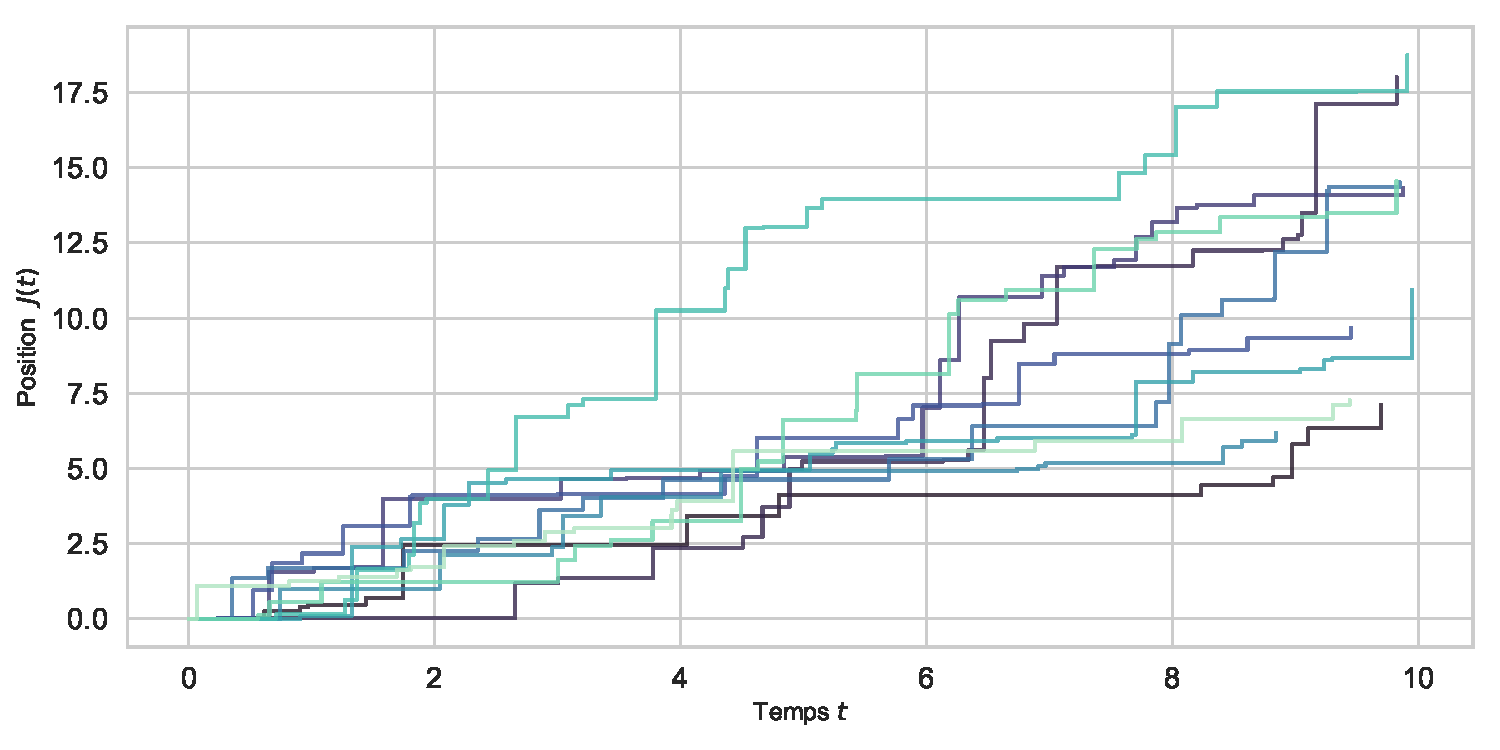
\includegraphics[width=0.9\linewidth]{img/intro/path_jump.pdf}
    \caption{Simulation de 10 trajectoire d'un processus de sauts pur $J(t)$}\label{fig:TrajJump}
\end{figure}
\FloatBarrier\clearpage

%%
%% ELEMENTS DE LA PROBLEMATIQUE
%%
\section{Éléments de la problématique}  % environ 3 pages

Comme évoqué précédemment, cette étude s'intéresse à des problèmes appliquées au processus \acl{CIR}. Il convient donc d'en donner une définition formelle.
\paragraph{Définition: Le processus \acl{CIR}}\mbox{}\\
Le processus \ac{CIR}~\cite{cox1985} est un processus d'Itô défini par l'équation différentielle stochastique suivante:
\begin{equation}
    dX(t) = a[b - X(t)]\,dt + \sigma \sqrt{X(t)}\,dW(t)
\end{equation}\label{cir_eq}
où:
\begin{itemize}
    \item $a \geq 0$ est le paramètre de vitesse;
    \item $b > 0$ représente la moyenne long-terme;
    \item $\sigma > 0$ est volatilité instantanée;
    \item $W(t)$ désigne un mouvement brownien standard.
\end{itemize}
Ce processus est particulièrement adapté à la modélisation des taux d'intérêt en raison de plusieurs propriétés clés:
\begin{itemize}
    \item Le terme de dérive $\mu(t, X(t)) \equiv \mu(X(t))= a[b - X(t)]$ induit un mécanisme de retour vers la moyenne $b$, avec une vitesse déterminée par $a$. Dans le contexte de modélisation des taux, cela reflète l'idée que ces derniers tendent à revenir vers un niveau de long terme après des déviations temporaires;
    \item Le terme de diffusion $\sigma(t, X(t))\equiv \sigma(X(t)) = \sigma \sqrt{X(t)}$ garantit la non-négativité du processus grâce à la racine carrée. Ceci est essentiel comme un taux négatif serait irréaliste dans de nombreux contextes économiques, en particulier pour les modèles de taux à court terme comme le CIR;
    \item Le comportement à proximité de zéro est gouverné par la \textit{condition de Feller}, selon laquelle:
    \[
    \mathds{P} \Big[ \exists\;t < \infty:X(t) = 0 \Big] = 1 \quad \text{si et seulement si} \quad \sigma^2 \geq 2ab
    \]
    Cela signifie que le processus peut atteindre zéro en un temps fini si la diffusion domine la dérive.
\end{itemize}
\begin{figure}[htb]
    \centering
    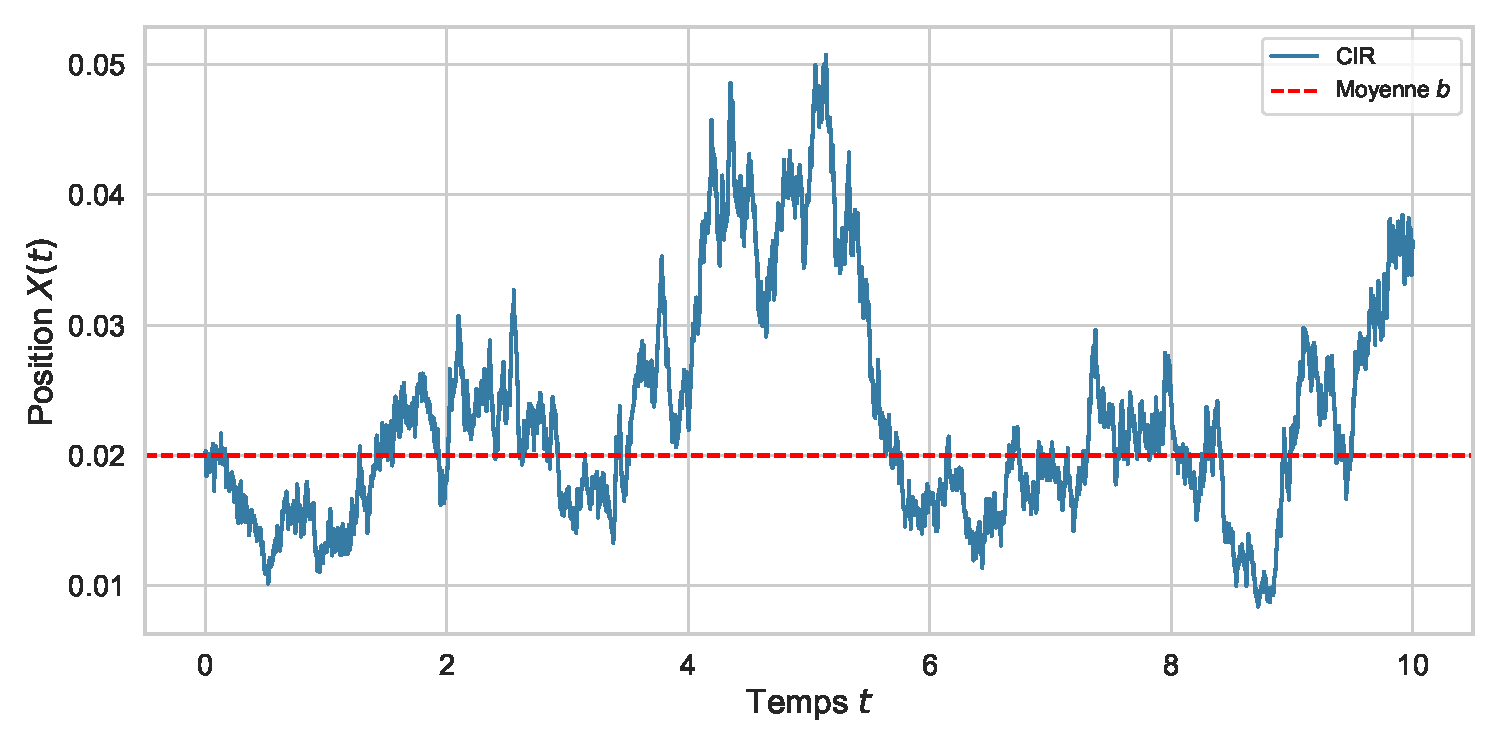
\includegraphics[width=0.9\linewidth]{img/intro/path_cir.pdf}
    \caption{Une trajectoire du processus \acs{CIR} avec $a=1$, $b=0.02$, $\sigma=0.1$}\label{fig:TrajCIR}
\end{figure}
\FloatBarrier Le prochain élément de problématique à introduire dans le cadre de cette étude est celui du \textit{temps de premier passage}.
\paragraph{Définition: Temps de premier passage}\mbox{}\\
Soit $\{X(t),\, t \geq 0\}$ un processus \acs{CIR}. Le \textit{temps de premier passage à deux frontières} est défini, pour un seuil $c > 0$, par:
\begin{equation}\label{fpt_definition}
    \tau(x) = \inf \left\{ t \geq 0: X(t) \notin (0, c) \,\middle|\, X(0) = x \in (0, c) \right\}
\end{equation}
Autrement dit, $\tau(x)$ correspond au premier instant où le processus atteint l'une des bornes de l'intervalle $(0, c)$. 

L'étude de ce temps d'arrêt est particulièrement pertinente dans le cadre du processus \acs{CIR}, pour plusieurs raisons:
\begin{itemize}
    \item \textbf{Modélisation du passage aux taux négatifs:} lors de la crise économique japonaise de 2016, des taux d'intérêt négatifs ont été instaurés pour stimuler l'activité. Or, le processus \acs{CIR}, à valeurs strictement positives, ne permet pas de modéliser ce phénomène. Introduire une barrière à zéro permet de considérer le franchissement de ce seuil, au-delà duquel les taux deviennent négatifs.
    \item \textbf{Surveillance des taux élevés:} en gestion des risques, il est crucial de modéliser l'éventualité d'une hausse brutale ou excessive des taux d'intérêt. L'introduction d'un seuil supérieur $c$ permet de caractériser ces situations critiques et de quantifier leur probabilité d'occurrence via le temps de franchissement.
\end{itemize}
\begin{figure}[htb]
    \centering
    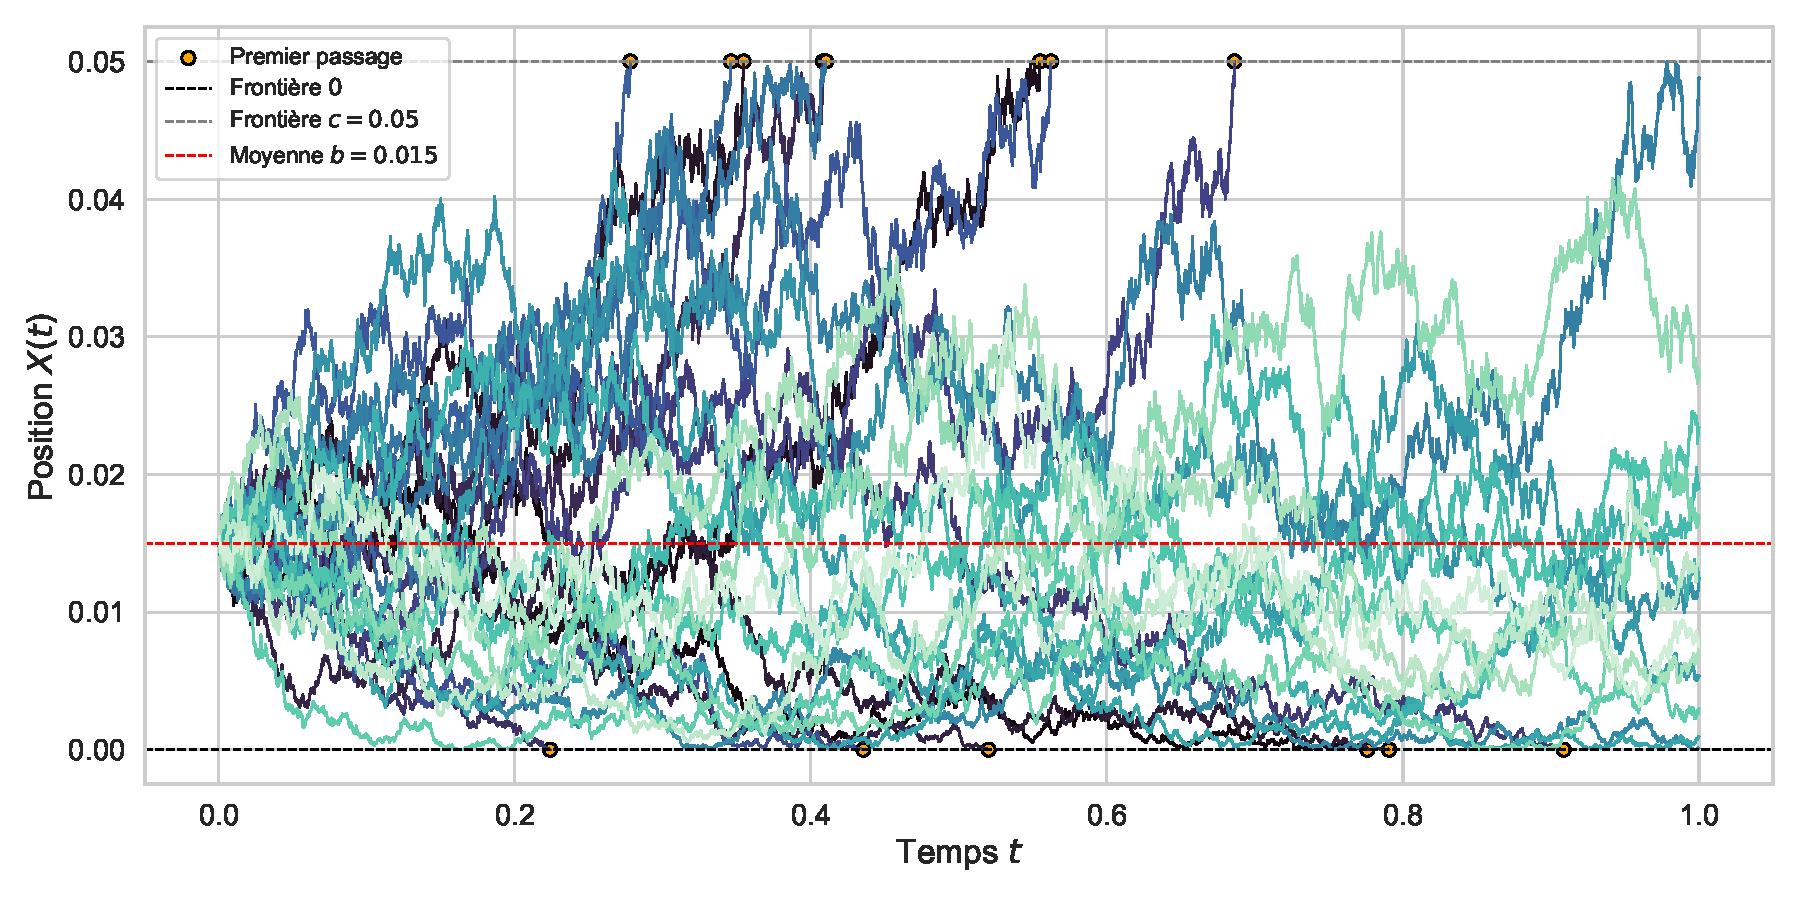
\includegraphics[width=0.9\linewidth]{img/intro/cir_first_passage.pdf}
    \caption{Simulations de 30 trajectoires du \acs{CIR} avec deux frontières absorbantes}\label{fig:FPTCIR}
\end{figure}
\FloatBarrier L'étude portera principalement sur le processus \acs{CIR}, noté $X(t)$, ainsi que sur la variable aléatoire associée au temps de premier passage $\tau(x)$.\\
Nous introduisons à présent les fonctions analytiques qui feront l'objet de l'analyse. La première est la \textit{fonction génératrice des moments}, outil central pour caractériser la distribution du temps d'arrêt.
\paragraph{Définition: \ac{FGM}}\mbox{}\\
La fonction génératrice des moments du temps de premier passage $\tau(x)$ est définie, pour tout $\alpha > 0$, par:
\begin{equation}\label{fgm}
    M(x;\alpha):= \mathds{E} \left[ e^{-\alpha \tau(x)} \right]
\end{equation}
Cette fonction permet de résumer l'information probabiliste sur la variable $\tau(x)$, en particulier sa distribution. De plus, elle encode l'ensemble des moments de $\tau(x)$, lorsque ceux-ci existent, via dérivation en $\alpha$. 

La deuxième fonction d'intérêt est celle du \textit{temps moyen de premier passage}, qui correspond à l'espérance de la variable aléatoire $\tau(x)$.
\paragraph{Définition: Temps Moyen de Premier Passage}\mbox{}\\
Le temps moyen de premier passage est défini par:
\begin{equation}\label{mean}
    m(x):= \mathds{E}[\tau(x)]
\end{equation}
Il représente le temps moyen que met le processus \acs{CIR}, partant d'un niveau initial $x \in (0,c)$, pour atteindre l'une des deux bornes de l'intervalle $(0,c)$.

La troisième fonction étudiée est celle de l'\textit{aire moyenne sous la trajectoire} jusqu'au temps de sortie.
\paragraph{Définition: Aire Moyenne}\mbox{}\\
La fonction d'aire moyenne est définie par:
\begin{equation}\label{area}
    A(x):= \mathds{E} \left[ \int_0^{\tau(x)} X(t)\,dt \right]
\end{equation}
En finance, l'aire moyenne peut représenter l'accumulation moyenne d'un taux d'intérêt à court terme jusqu'à un événement de sortie. Elle intervient également dans la tarification d'options asiatiques avec barrière, où le \textit{payoff} dépend de l'intégrale temporelle du sous-jacent avant la sortie d'un intervalle donné.

La quatrième fonction étudiée est celle de la probabilité toucher la frontière inférieure.
\paragraph{Définition: Probabilité de Sortie en Zéro}\mbox{}\\
La fonction de probabilité de sortie est définie par:
\begin{equation}\label{zero_exit_probability}
    p(x):=\mathds{P}[X(\tau(x))=0]
\end{equation}
Elle caractérise la probabilité que le processus, partant d'une position initiale $x$, sorte de l'intervalle $(0,c)$ par le bas. Cette quantité peut être utilisée pour quantifier un risque de ruine, de défaut, ou encore d'apparition de taux négatifs (si le contexte économique le permet).

La cinquième fonction étudiée est celle du \textit{dépassement moyen}, en ajoutant des sauts au \acs{CIR}.
\paragraph{Définition: Dépassement Moyen}\mbox{}\\
La fonction dépassement moyen est définie par: 
\begin{equation}\label{overshoot}
    D(x)=\mathds{E}\left[(X(\tau(x))-c)_+\right]
\end{equation}
Elle quantifie le dépassement moyen au-dessus de la frontière \( c \), à partir d'une condition initiale \( X(0) = x \in (0, c) \). Il est essentiel de souligner que cette fonction ne présente un intérêt que dans le cas où le processus comporte des sauts. En effet, dans le cadre purement continu, la trajectoire atteint la frontière exactement, sans possibilité de la franchir.
\begin{figure}[htb]
    \centering
    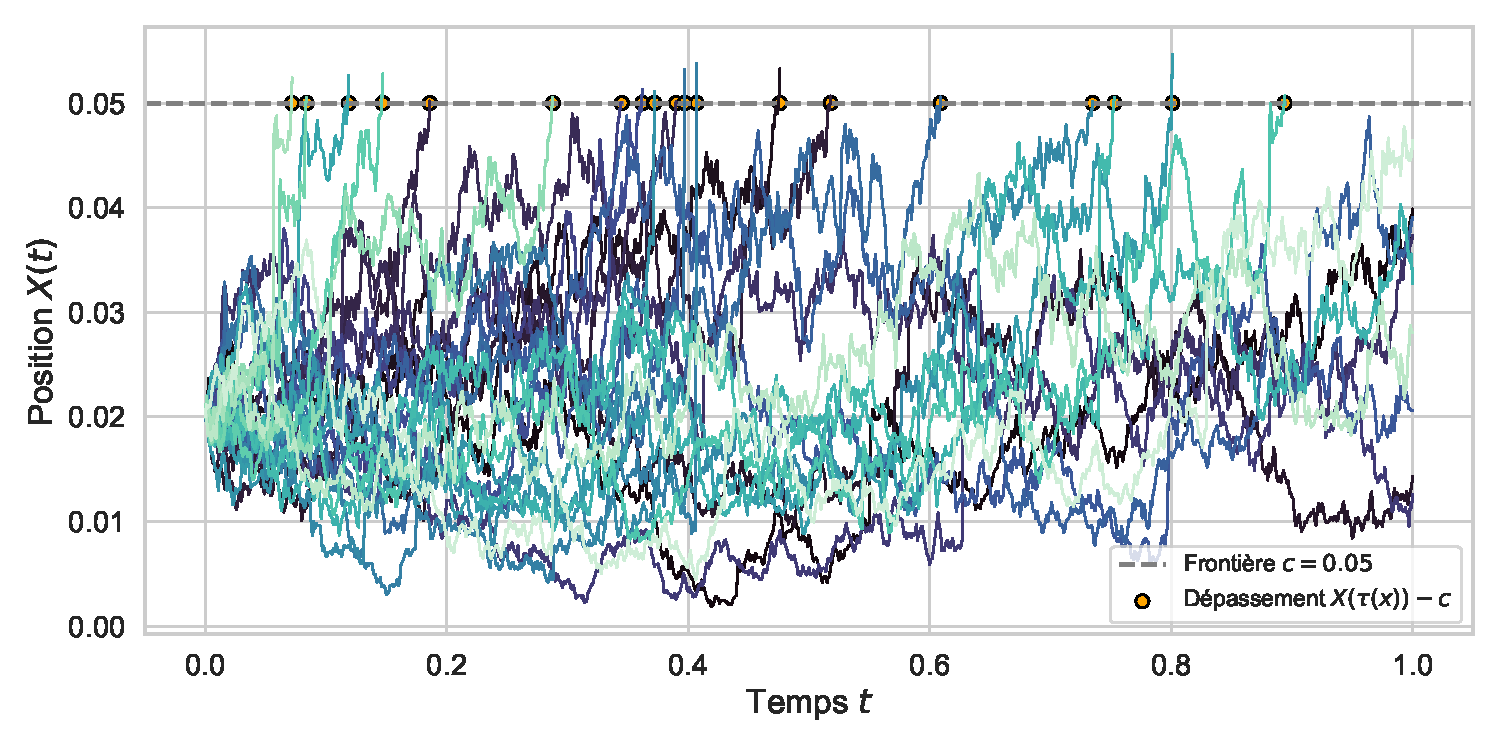
\includegraphics[width=0.9\linewidth]{img/intro/overshoot.pdf}
    \caption{Simulations de 30 trajectoires du \acs{CIR} avec sauts dépassants la frontière $c$}\label{fig:OvershootViz}
\end{figure}
\FloatBarrier Ce type de quantité apparaît notamment dans la valorisation de produits financiers path-dependent, tels que les options lookback ou les produits structurés à barrière, où le dépassement moyen modélise l'espérance de gain associée au franchissement d'un niveau critique par le sous-jacent. 

En complément de l'étude des temps de premier passage, ce mémoire s'intéresse également à un problème de \textit{commande optimale stochastique} appliqué au processus \acs{CIR}.\\
\paragraph{Définition: Problème de commande optimale \textemdash~Homing Problem}\label{definition_optimal_control}\mbox{}\\
Le \textit{Homing problem} consiste à piloter un processus stochastique dynamiquement jusqu'à ce qu'il atteigne un ensemble d'arrêt donné, tout en optimisant un objectif. La configuration étudiée dans ce mémoire correspond à un processus \acs{CIR} contrôlé \( \{X_u(t),\, t \geq 0\} \) évoluant dans l'intervalle \( (0, c) \), avec un arrêt déclenché dès que la trajectoire atteint l'une des deux frontières. Ce processus est défini par:
\begin{equation}\label{controlled_process}
    dX_u(t) = a[b - X_u(t)]dt + b[X_u(t)]u[X_u(t)]dt + \sigma \sqrt{X_u(t)} dW(t)
\end{equation}
où \( u(\cdot) \) est une stratégie de contrôle.

Le processus est contrôlé jusqu'à l'instant d'arrêt $\tau(x)$ défini précédemment (\ref{fpt_definition}).
Par ailleurs, l'objectif est de minimiser une fonction coût de type intégral, définie par:
\begin{equation}\label{cost_function}
    J(x) := \int_0^{\tau(x)} \left( \frac{1}{2}q[X_u(t)]u^2[X_u(t)] + r[X_u(t)] \right) dt
\end{equation}
où:
\begin{itemize}
    \item \( r(x) \neq 0 \) est le coût d'état (non associé au contrôle);
    \item \( b(x) \neq 0 \) est le coût du contrôle appliqué;
    \item \( q(x) > 0 \) est un poids pénalisant l'intensité du contrôle.
\end{itemize}
Le problème consiste à déterminer une stratégie optimale \( u^*(x) \) minimisant ce coût. La fonction valeur associée au problème s'écrit:
\begin{equation}\label{value_function}
    F(x) := \inf_{\underset{0 \leq t \leq \tau(x)}{u[X_u(t)]}} \mathds{E}[J(x)]
\end{equation}
La figure ci-dessous illustre l'effet d'une stratégie de contrôle sur la dynamique du processus. Dans cet exemple, la commande utilisée est constante et positive ($u(x)\equiv5$), ce qui génère une force dirigée vers la frontière supérieure \( c \) et accélère ainsi la sortie du processus par le haut.
\begin{figure}[htb]
    \centering
    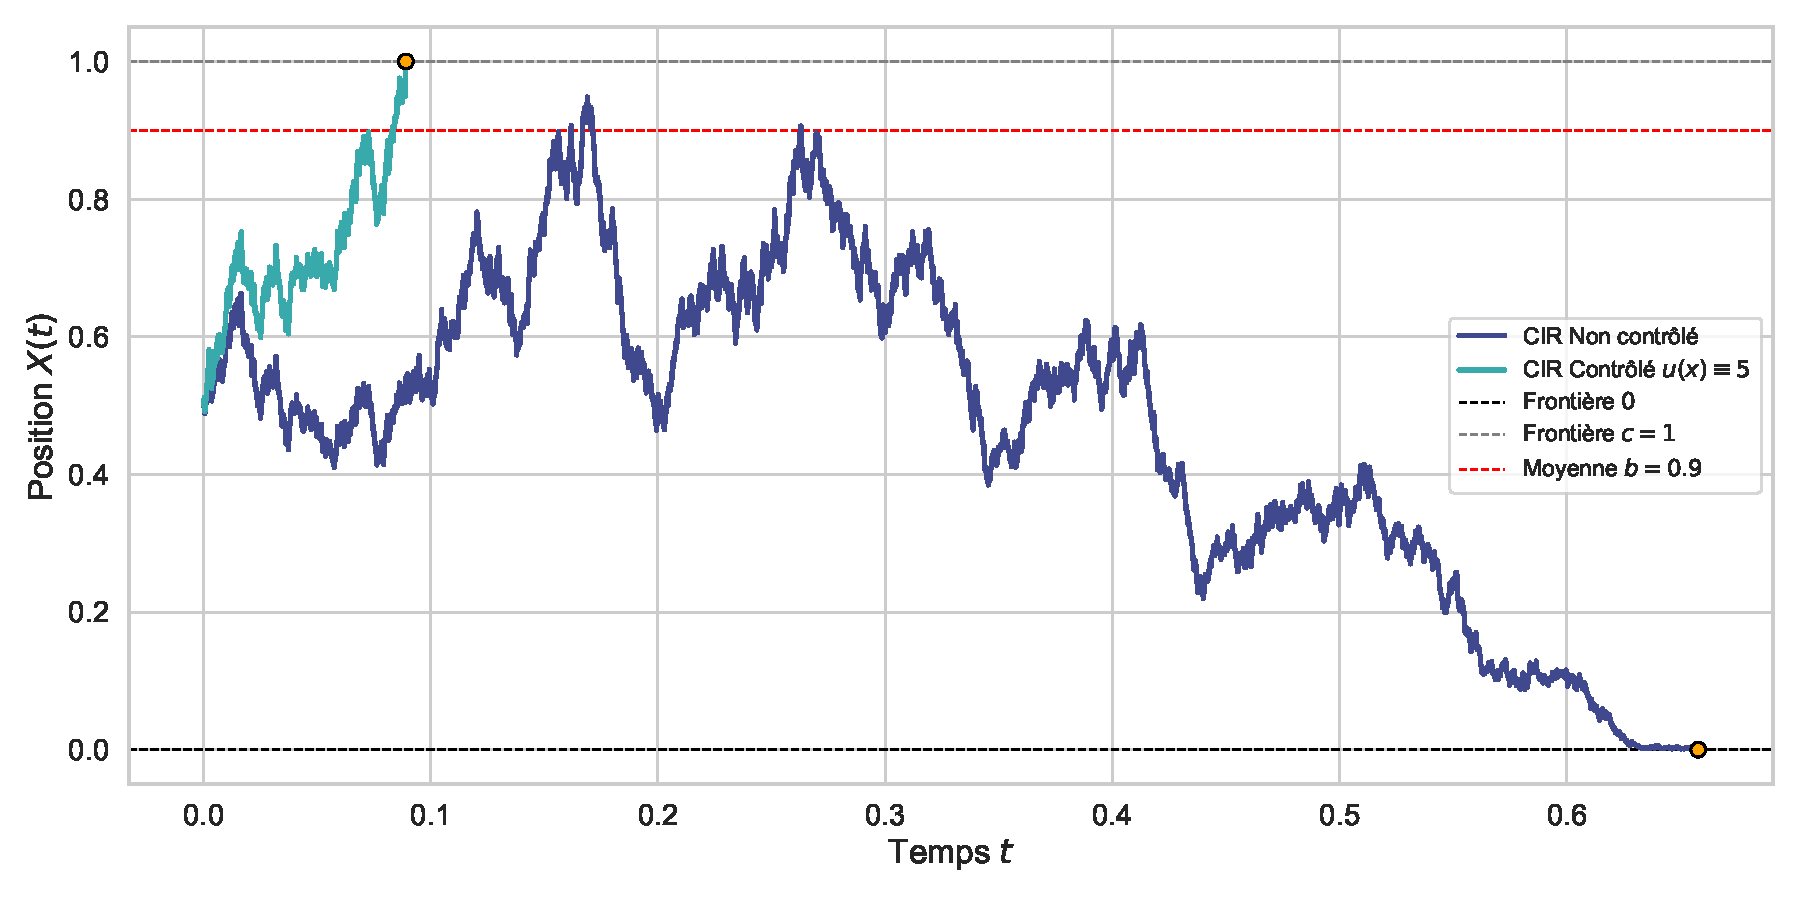
\includegraphics[width=0.9\linewidth]{img/intro/control.pdf}
    \caption{Simulations de deux trajectoires du CIR avec et sans contrôle}\label{fig:ControlViz}
\end{figure}
\FloatBarrier



\clearpage

%%
%% OBJECTIFS DE RECHERCHE / RESEARCH OBJECTIVES
%%
\section{Objectifs de recherche}  % 0.5 page

Après avoir exposé les fondements théoriques de l'étude, nous pouvons désormais énoncer précisément les objectifs poursuivis dans ce mémoire. Ceux-ci se répartissent en deux volets: l'analyse des temps de premier passage pour le processus \acs{CIR} en diffusion pure, puis l'étude de son extension avec sauts.
\paragraph{Objectifs pour le processus de diffusion}
\begin{itemize}
    \item Obtenir une expression explicite de la fonction génératrice des moments du temps de premier passage à deux frontières \( M(x;\alpha) = \mathds{E}[e^{-\alpha \tau(x)}] \);
    \item Expliciter une formule analytique pour le temps moyen de premier passage, \( m(x) = \mathds{E}[\tau(x)] \), pour une entrée initiale \( x \in (0,c) \);
    \item Déduire l'aire moyenne sous la trajectoire $A(x)$ jusqu'au franchissement de l'intervalle \( (0,c) \);
    \item Résoudre différentes formes d'un problème de commande optimale associé au processus, en déterminant la fonction valeur \( F(x) = \underset{u}{\inf}\,\mathds{E}[J(x)] \), ainsi que la politique de contrôle optimal $u^*(x)$.
\end{itemize}
\paragraph{Objectifs pour le processus de diffusion avec sauts}
\begin{itemize}
    \item Obtenir une expression analytique du temps moyen de sortie dans ce nouveau cadre, en tenant compte de l'impact des sauts sur la dynamique du processus;
    \item Établir une forme explicite de la probabilité de sortie par zéro:
    \(
    p(x) = \mathds{P}[X(\tau(x)) = 0],
    \)
    dans le cas de sauts uniformes descendants;
    \item Déterminer le dépassement moyen à l'instant du franchissement supérieur \( c \), défini par:
    \(
    D(x) = \mathds{E}[(X(\tau(x)) - c)_+]
    \)
    afin d'évaluer l'intensité des excursions au-delà de la borne supérieure, dans le cas de sauts exponentiels ascendants.
\end{itemize}


%%
%% PLAN DU MEMOIRE / THESIS OUTLINE
%%
\section{Plan du mémoire}  % 0.5 page
Afin de répondre aux objectifs de recherche définis précédemment, ce mémoire est structuré de la manière suivante.

Dans un premier temps, une revue de la littérature est proposée afin de replacer l'étude dans le cadre des travaux existants sur les temps de premier passage et les problèmes de dépassement, avec une attention particulière portée au processus \acs{CIR} et à ses extensions.

La suite du mémoire est consacrée à l'étude analytique des fonctions caractéristiques associées au processus. L'analyse se divise en deux parties distinctes: 
\begin{itemize}
    \item la première porte sur le processus \acs{CIR} en diffusion pure;
    \item la seconde examine sa version modifiée par l'introduction de sauts discrets.
\end{itemize}
Dans chaque cas, les équations différentielles correspondantes sont établies puis résolues.

Une section est ensuite dédiée à l'analyse des résultats obtenus. Cette dernière permet de vérifier la cohérence des solutions, d'en évaluer la sensibilité aux paramètres du modèle, et de comparer les dynamiques avec et sans sauts.

Enfin, la conclusion synthétise les contributions principales du mémoire, discute les limites de l'approche adoptée, et propose plusieurs pistes d'approfondissement pour des travaux futurs.

